\section{Рабочий проект}


\subsection{Спецификация компонентов и классов системы}

\subsubsection{Спецификация класса User}
User (Компонент управления пользователями) \\
Описание: Представляет пользователя системы (студента или преподавателя). Используется для аутентификации, управления ролями и отслеживания активности пользователей. Расширяет встроенную модель Django AbstractUser.

Валидация данных: 
\begin{itemize}
	\item поля username, email, password валидируются через встроенные механизмы Django (django.contrib.auth); 
	\item поля isstudent и isteacher — булевы, только одно из них может быть True (проверяется на уровне форм, например, StudentSignUpForm); 
\end{itemize}

Безопасность: 
\begin{itemize}
	\item доступ к данным пользователя ограничен через декораторы (loginrequired, teacherrequired, studentrequired) в представлениях; 
\end{itemize}

Уведомления: 
\begin{itemize}
	\item уведомления о действиях пользователя (например, регистрация, смена пароля) отображаются через Django messages framework в представлениях; 
\end{itemize}

Основные методы: 
\begin{itemize}
	\item str(): возвращает имя пользователя (username); 
	\item hasperm(perm, obj=None): проверяет права доступа пользователя; 
	\item save(): переопределяется для автоматической проверки ролей (isstudent, isteacher) перед сохранением; 
\end{itemize}

Зависимости: 
\begin{itemize}
	\item встроенная модель Django (django.contrib.auth.models.AbstractUser); 
	\item связан с моделями Enrollment, StudentProgress, UserAchievement через внешние ключи; 
	\item используется в формах (StudentSignUpForm, TeacherSignUpForm) и представлениях (StudentSignUpView, TeacherSignUpView); 
\end{itemize}

Таблица 4.1 – Данные класса User \\
\begin{tabular}{|p{4cm}|p{8cm}|}
	\hline
	Данные & Описание \\
	\hline
	username & уникальное имя пользователя; \\
	email & электронная почта пользователя; \\
	password & хэшированный пароль пользователя; \\
	isstudent & булево поле, указывающее, является ли пользователь студентом; \\
	isteacher & булево поле, указывающее, является ли пользователь преподавателем; \\
	fields & поля модели User, доступные для заполнения (username, email, password, isstudent, isteacher); \\
	\hline
\end{tabular}

Таблица 4.2 – Методы класса User \\
\begin{tabular}{|p{4cm}|p{8cm}|}
	\hline
	Метод & Описание \\
	\hline
	str() & возвращает имя пользователя (username); \\
	hasperm(perm, obj=None) & проверяет права доступа пользователя на основе роли и разрешений; \\
	save() & переопределяет сохранение для проверки ролей (isstudent, isteacher); \\
	\hline
\end{tabular}

\subsubsection{Спецификация класса Course}
Course (Компонент управления курсами) \\
Описание: Представляет учебный курс, созданный преподавателем. Хранит информацию о названии, описании, изображении и статусе публикации. Используется для организации уроков и тестов.

Валидация данных: 
\begin{itemize}
	\item поля title, description валидируются через Django-формы (CourseForm); 
	\item поле image проверяется на корректный формат (например, JPEG, PNG) через FileField валидаторы; 
\end{itemize}

Связи: 
\begin{itemize}
	\item связан с моделью User через поле creator (внешний ключ); 
	\item связан с моделями Lesson и Enrollment через внешние ключи (course); 
\end{itemize}

Безопасность: 
\begin{itemize}
	\item доступ к редактированию курса ограничен через проверку creator в представлениях (например, CourseUpdateView); 
	\item студенты могут просматривать только опубликованные курсы (isactive=True); 
\end{itemize}

Уведомления: 
\begin{itemize}
	\item уведомления о создании или обновлении курса отображаются через Django messages framework в представлениях (например, "Курс успешно обновлён"); 
\end{itemize}

Основные методы: 
\begin{itemize}
	\item str(): возвращает название курса (title); 
	\item getabsoluteurl(): возвращает URL курса для маршрутизации (например, /courses/<id>/); 
	\item save(): переопределяет сохранение для обработки изображения; 
\end{itemize}

Зависимости: 
\begin{itemize}
	\item взаимодействует с моделями Lesson, Test и Enrollment; 
	\item используется в шаблонах (coursedetail.html, courseform.html) с CKEditor для редактирования описания; 
	\item зависит от defaultstorage для хранения изображений; 
\end{itemize}

Таблица 4.3 – Данные класса Course \\
\begin{tabular}{|p{4cm}|p{8cm}|}
	\hline
	Данные & Описание \\
	\hline
	title & название курса; \\
	description & описание курса (форматируется через CKEditor); \\
	image & изображение курса (FileField); \\
	isactive & булево поле, указывающее статус публикации курса; \\
	creator & внешний ключ на User (преподаватель, создавший курс); \\
	fields & поля модели Course, доступные для заполнения (title, description, image, isactive, creator); \\
	\hline
\end{tabular}

Таблица 4.4 – Методы класса Course \\
\begin{tabular}{|p{4cm}|p{8cm}|}
	\hline
	Метод & Описание \\
	\hline
	str() & возвращает название курса (title); \\
	getabsoluteurl() & возвращает URL курса для маршрутизации; \\
	save() & переопределяет сохранение для обработки изображения; \\
	\hline
\end{tabular}

\subsubsection{Спецификация класса Lesson}
Lesson (Компонент управления уроками) \\
Описание: Представляет урок в рамках курса. Хранит информацию о заголовке, описании, содержимом, видео, упражнении и порядке отображения. Используется для структурирования учебного материала.

Валидация данных: 
\begin{itemize}
	\item поля title, description, content валидируются через Django-формы (LessonForm); 
	\item поле videourl проверяется на корректность через валидаторы Django; 
\end{itemize}

Связи: 
\begin{itemize}
	\item связан с моделью Course через поле course (внешний ключ); 
	\item связан с моделями Test и StudentProgress через внешние ключи (lesson); 
\end{itemize}

Безопасность: 
\begin{itemize}
	\item доступ к редактированию урока ограничен через проверку creator курса в представлениях (например, LessonUpdateView); 
	\item студенты имеют доступ только к опубликованным урокам (ispublished=True); 
\end{itemize}

Уведомления: 
\begin{itemize}
	\item уведомления о создании или обновлении урока отображаются через Django messages framework (например, "Урок успешно добавлен"); 
\end{itemize}

Основные методы: 
\begin{itemize}
	\item str(): возвращает название урока (title); 
	\item save(): переопределяет сохранение для проверки порядка (order); 
\end{itemize}

Зависимости: 
\begin{itemize}
	\item взаимодействует с моделями Course, Test и StudentProgress; 
	\item используется в шаблонах (lessondetail.html) с CKEditor для редактирования контента; 
\end{itemize}

Таблица 4.5 – Данные класса Lesson \\
\begin{tabular}{|p{4cm}|p{8cm}|}
	\hline
	Данные & Описание \\
	\hline
	title & название урока; \\
	description & описание урока; \\
	content & содержимое урока (форматируется через CKEditor); \\
	videourl & ссылка на видео урока; \\
	order & порядок урока в курсе; \\
	ispublished & булево поле, указывающее статус публикации урока; \\
	exercise & интерактивное упражнение урока; \\
	expectedresult & ожидаемый результат упражнения; \\
	course & внешний ключ на Course; \\
	fields & поля модели Lesson, доступные для заполнения (title, description, content, videourl, order, ispublished, exercise, expectedresult, course); \\
	\hline
\end{tabular}

Таблица 4.6 – Методы класса Lesson \\
\begin{tabular}{|p{4cm}|p{8cm}|}
	\hline
	Метод & Описание \\
	\hline
	str() & возвращает название урока (title); \\
	save() & переопределяет сохранение для проверки порядка (order); \\
	\hline
\end{tabular}

\subsubsection{Спецификация класса Test}
Test (Компонент управления тестами) \\
Описание: Представляет тест, связанный с уроком. Хранит информацию о названии, описании, проходном балле и статусе активности. Используется для проверки знаний студентов.

Валидация данных: 
\begin{itemize}
	\item поля title, description валидируются через Django-формы (TestForm); 
	\item поле passingscore проверяется на положительное значение через валидаторы;
\end{itemize}

Связи: 
\begin{itemize}
	\item связан с моделью Lesson через поле lesson (внешний ключ); 
	\item связан с моделями Question и TestResult через внешние ключи (test); 
\end{itemize}

Безопасность: 
\begin{itemize}
	\item доступ к редактированию теста ограничен через проверку creator урока в представлениях (например, createtest); 
	\item студенты могут проходить только активные тесты (isactive=True); 
\end{itemize}

Уведомления: 
\begin{itemize}
	\item уведомления о создании теста отображаются через Django messages framework (например, "Тест успешно создан"); 
\end{itemize}

Основные методы: 
\begin{itemize}
	\item str(): возвращает название теста (title); 
	\item save(): переопределяет сохранение для проверки passingscore; 
\end{itemize}

Зависимости: 
\begin{itemize}
	\item взаимодействует с моделями Lesson, Question и TestResult; 
	\item используется в шаблонах (testform.html) и представлениях (createtest); 
\end{itemize}

Таблица 4.7 – Данные класса Test \\
\begin{tabular}{|p{4cm}|p{8cm}|}
	\hline
	Данные & Описание \\
	\hline
	title & название теста; \\
	description & описание теста; \\
	passingscore & проходной балл теста; \\
	isactive & булево поле, указывающее статус активности теста; \\
	lesson & внешний ключ на Lesson; \\
	fields & поля модели Test, доступные для заполнения (title, description, passingscore, isactive, lesson); \\
	\hline
\end{tabular}

Таблица 4.8 – Методы класса Test \\
\begin{tabular}{|p{4cm}|p{8cm}|}
	\hline
	Метод & Описание \\
	\hline
	str() & возвращает название теста (title); \\
	save() & переопределяет сохранение для проверки passingscore; \\
	\hline
\end{tabular}

\subsubsection{Спецификация класса Question}
Question (Компонент управления вопросами теста) \\
Описание: Представляет вопрос в тесте. Хранит текст вопроса, тип вопроса (одиночный, множественный, текстовый) и баллы за правильный ответ.

Валидация данных: 
\begin{itemize}
	\item поле text валидируется через Django-формы (QuestionForm); 
	\item поле questiontype проверяется на допустимые значения (single, multiple, text); 
	\item поле points проверяется на положительное значение; 
\end{itemize}

Связи: 
\begin{itemize}
	\item связан с моделью Test через поле test (внешний ключ); 
	\item связан с моделью Answer через внешний ключ (question); 
\end{itemize}

Безопасность: 
\begin{itemize}
	\item доступ к редактированию вопроса ограничен через проверку creator урока в представлениях (например, addquestion); 
\end{itemize}

Уведомления: 
\begin{itemize}
	\item уведомления о добавлении вопроса отображаются через Django messages framework (например, "Вопрос успешно добавлен"); 
\end{itemize}

Основные методы: 
\begin{itemize}
	\item str(): возвращает текст вопроса (text); 
	\item save(): переопределяет сохранение для проверки questiontype и points; 
\end{itemize}

Зависимости: 
\begin{itemize}
	\item взаимодействует с моделями Test и Answer; 
	\item используется в шаблонах (questionform.html) и представлениях (addquestion); 
\end{itemize}

Таблица 4.9 – Данные класса Question \\
\begin{tabular}{|p{4cm}|p{8cm}|}
	\hline
	Данные & Описание \\
	\hline
	text & текст вопроса; \\
	questiontype & тип вопроса (single, multiple, text); \\
	points & баллы за правильный ответ; \\
	test & внешний ключ на Test; \\
	fields & поля модели Question, доступные для заполнения (text, questiontype, points, test); \\
	\hline
\end{tabular}

Таблица 4.10 – Методы класса Question \\
\begin{tabular}{|p{4cm}|p{8cm}|}
	\hline
	Метод & Описание \\
	\hline
	str() & возвращает текст вопроса (text); \\
	save() & переопределяет сохранение для проверки questiontype и points; \\
	\hline
\end{tabular}

\subsubsection{Спецификация класса Answer}
Answer (Компонент управления ответами на вопросы) \\
Описание: Представляет вариант ответа на вопрос в тесте. Хранит текст ответа, флаг правильности и порядок отображения.

Валидация данных: 
\begin{itemize}
	\item поле text валидируется через Django-формы (AnswerForm); 
	\item поле iscorrect — булево, проверяется на уровне формы; 
	\item поле order проверяется на положительное значение; 
\end{itemize}

Связи: 
\begin{itemize}
	\item связан с моделью Question через поле question (внешний ключ); 
	\item используется в TestResult для хранения выбранных ответов; 
\end{itemize}

Безопасность: 
\begin{itemize}
	\item доступ к редактированию ответа ограничен через проверку creator урока в представлениях (например, AnswerCreateView); 
\end{itemize}

Уведомления: 
\begin{itemize}
	\item уведомления о добавлении ответа отображаются через Django messages framework (например, "Ответ успешно добавлен"); 
\end{itemize}

Основные методы: 
\begin{itemize}
	\item str(): возвращает текст ответа (text); 
	\item save(): переопределяет сохранение для проверки iscorrect и order; 
\end{itemize}

Зависимости: 
\begin{itemize}
	\item взаимодействует с моделями Question и TestResult; 
	\item используется в шаблонах (answerform.html) и представлениях (AnswerCreateView); 
\end{itemize}

Таблица 4.11 – Данные класса Answer \\
\begin{tabular}{|p{4cm}|p{8cm}|}
	\hline
	Данные & Описание \\
	\hline
	text & текст ответа; \\
	iscorrect & булево поле, указывающее правильность ответа; \\
	order & порядок отображения ответа; \\
	question & внешний ключ на Question; \\
	fields & поля модели Answer, доступные для заполнения (text, iscorrect, order, question); \\
	\hline
\end{tabular}

Таблица 4.12 – Методы класса Answer \\
\begin{tabular}{|p{4cm}|p{8cm}|}
	\hline
	Метод & Описание \\
	\hline
	str() & возвращает текст ответа (text); \\
	save() & переопределяет сохранение для проверки iscorrect и order; \\
	\hline
\end{tabular}

\subsubsection{Спецификация класса TestResult}
TestResult (Компонент управления результатами тестов) \\
Описание: Хранит результаты тестов, пройденных студентами. Содержит информацию о студенте, уроке, баллах, ответах и дате завершения.

Валидация данных: 
\begin{itemize}
	\item поле score проверяется на положительное значение и соответствие максимальным баллам теста; 
	\item поле answers валидируется через Django-формы (TestSubmissionForm); 
\end{itemize}

Связи: \\
\begin{itemize}
	\item связан с моделью User через поле student (внешний ключ); 
	\item связан с моделью Lesson через поле lesson (внешний ключ); 
	\item хранит ссылки на выбранные ответы (answers); 
\end{itemize}

Безопасность: 
\begin{itemize}
	\item доступ к результатам ограничен через проверку student или creator урока в представлениях (например, testresult); 
\end{itemize}

Уведомления: 
\begin{itemize}
	\item уведомления о прохождении теста отображаются через Django messages framework (например, "Тест успешно пройден"); 
\end{itemize}

Основные методы: 
\begin{itemize}
	\item str(): возвращает данные о результате (например, "Результат студента X по уроку Y"); 
	\item save(): переопределяет сохранение для пересчёта score на основе answers; 
\end{itemize}

Зависимости: 
\begin{itemize}
	\item взаимодействует с моделями User, Lesson и Answer; 
	\item используется в шаблонах (testresult.html) и представлениях (testresult); 
\end{itemize}

Таблица 4.13 – Данные класса TestResult \\
\begin{tabular}{|p{4cm}|p{8cm}|}
	\hline
	Данные & Описание \\
	\hline
	student & внешний ключ на User (студент); \\
	lesson & внешний ключ на Lesson; \\
	score & баллы, полученные за тест; \\
	answers & выбранные ответы студента; \\
	attempts & количество попыток прохождения теста; \\
	completedat & дата и время завершения теста; \\
	fields & поля модели TestResult, доступные для заполнения (student, lesson, score, answers, attempts, completedat); \\
	\hline
\end{tabular}

Таблица 4.14 – Методы класса TestResult \\
\begin{tabular}{|p{4cm}|p{8cm}|}
	\hline
	Метод & Описание \\
	\hline
	str() & возвращает данные о результате (например, "Результат студента X по уроку Y"); \\
	save() & переопределяет сохранение для пересчёта score на основе answers; \\
	\hline
\end{tabular}

\subsubsection{Спецификация класса Enrollment}
Enrollment (Компонент управления записями на курсы) \\
Описание: Хранит информацию о записи студента на курс. Связывает студента и курс для отслеживания участия.

Валидация данных: 
\begin{itemize}
	\item поля student и course проверяются на уникальность (студент не может записаться на один курс дважды); 
	\item проверка осуществляется через Django ORM (uniquetogether); 
\end{itemize}

Связи: 
\begin{itemize}
	\item связан с моделью User через поле student (внешний ключ); 
	\item связан с моделью Course через поле course (внешний ключ); 
\end{itemize}

Безопасность: 
\begin{itemize}
	\item доступ к записи ограничен через проверку student в представлениях (например, enrollcourse); 
	\item преподаватели могут просматривать записи через teacherdashboard; 
\end{itemize}

Уведомления: 
\begin{itemize}
	\item уведомления о записи на курс отображаются через Django messages framework (например, "Вы записаны на курс"); 
\end{itemize}

Основные методы: 
\begin{itemize}
	\item str(): возвращает данные о записи (например, "Студент X записан на курс Y"); 
	\item save(): переопределяет сохранение для проверки уникальности записи; 
\end{itemize}

Зависимости: 
\begin{itemize}
	\item взаимодействует с моделями User и Course; 
	\item используется в представлениях (enrollcourse, unenrollcourse); 
\end{itemize}

Таблица 4.15 – Данные класса Enrollment \\
\begin{tabular}{|p{4cm}|p{8cm}|}
	\hline
	Данные & Описание \\
	\hline
	student & внешний ключ на User (студент); \\
	course & внешний ключ на Course; \\
	fields & поля модели Enrollment, доступные для заполнения (student, course); \\
	\hline
\end{tabular}

Таблица 4.16 – Методы класса Enrollment \\
\begin{tabular}{|p{4cm}|p{8cm}|}
	\hline
	Метод & Описание \\
	\hline
	str() & возвращает данные о записи (например, "Студент X записан на курс Y"); \\
	save() & переопределяет сохранение для проверки уникальности записи; \\
	\hline
\end{tabular}

\subsubsection{Спецификация класса StudentProgress}
StudentProgress (Компонент управления прогрессом студентов) \\
Описание: Хранит информацию о прогрессе студента по урокам. Отмечает завершённость уроков и дату завершения.

Валидация данных: 
\begin{itemize}
	\item поле completed — булево, устанавливается через представления (например, completelesson); 
	\item поле completedat автоматически заполняется текущей датой при установке completed=True; 
\end{itemize}

Связи: 
\begin{itemize}
	\item связан с моделью User через поле student (внешний ключ); 
	\item связан с моделью Lesson через поле lesson (внешний ключ); 
\end{itemize}

Безопасность: 
\begin{itemize}
	\item доступ к прогрессу ограничен через проверку student в представлениях (например, studentdashboard); 
\end{itemize}

Уведомления: 
\begin{itemize}
	\item уведомления о завершении урока отображаются через Django messages framework (например, "Урок успешно завершён"); 
\end{itemize}

Основные методы: 
\begin{itemize}
	\item str(): возвращает данные о прогрессе (например, "Прогресс студента X по уроку Y"); 
	\item save(): переопределяет сохранение для установки completedat; 
\end{itemize}

Зависимости: 
\begin{itemize}
	\item взаимодействует с моделями User и Lesson;
	\item используется в представлениях (completelesson, studentdashboard); 
\end{itemize}

Таблица 4.17 – Данные класса StudentProgress \\
\begin{tabular}{|p{4cm}|p{8cm}|}
	\hline
	Данные & Описание \\
	\hline
	student & внешний ключ на User (студент); \\
	lesson & внешний ключ на Lesson; \\
	completed & булево поле, указывающее завершённость урока; \\
	completedat & дата завершения урока; \\
	fields & поля модели StudentProgress, доступные для заполнения (student, lesson, completed, completedat); \\
	\hline
\end{tabular}

Таблица 4.18 – Методы класса StudentProgress \\
\begin{tabular}{|p{4cm}|p{8cm}|}
	\hline
	Метод & Описание \\
	\hline
	str() & возвращает данные о прогрессе (например, "Прогресс студента X по уроку Y"); \\
	save() & переопределяет сохранение для установки completedat; \\
	\hline
\end{tabular}

\subsubsection{Спецификация класса Achievement}
Achievement (Компонент управления достижениями) \\
Описание: Хранит информацию о достижениях, которые могут быть присвоены студентам (например, "Первый завершённый урок"). Содержит название и описание достижения.

Валидация данных: 
\begin{itemize}
	\item поля title, description валидируются через Django-формы (AchievementForm); 
	\item проверка уникальности title осуществляется через Django ORM; 
\end{itemize}

Связи: 
\begin{itemize}
	\item связан с моделью UserAchievement через внешний ключ (achievement); 
\end{itemize}

Безопасность: 
\begin{itemize}
	\item доступ к редактированию достижений ограничен через проверку isstaff в представлениях (для администраторов); 
\end{itemize}

Уведомления: 
\begin{itemize}
	\item уведомления о создании достижения отображаются через Django messages framework (например, "Достижение успешно создано"); 
\end{itemize}

Основные методы: 
\begin{itemize}
	\item str(): возвращает название достижения (title); 
	\item save(): переопределяет сохранение для проверки уникальности title; 
\end{itemize}

Зависимости: 
\begin{itemize}
	\item взаимодействует с моделью UserAchievement; 
	\item используется в представлениях (studentdashboard) для отображения достижений; 
\end{itemize}

Таблица 4.19 – Данные класса Achievement \\
\begin{tabular}{|p{4cm}|p{8cm}|}
	\hline
	Данные & Описание \\
	\hline
	title & название достижения; \\
	description & описание достижения; \\
	fields & поля модели Achievement, доступные для заполнения (title, description); \\
	\hline
\end{tabular}

Таблица 4.20 – Методы класса Achievement \\
\begin{tabular}{|p{4cm}|p{8cm}|}
	\hline
	Метод & Описание \\
	\hline
	str() & возвращает название достижения (title); \\
	save() & переопределяет сохранение для проверки уникальности title; \\
	\hline
\end{tabular}

\subsubsection{Спецификация класса UserAchievement}
UserAchievement (Компонент управления достижениями пользователей) \\
Описание: Хранит связь между пользователями и их достижениями. Используется для отслеживания, какие достижения были присвоены студентам.

Валидация данных: 
\begin{itemize}
	\item поля user и achievement проверяются на уникальность (один пользователь не может получить одно достижение дважды); 
	\item проверка осуществляется через Django ORM (uniquetogether); 
\end{itemize}

Связи: 
\begin{itemize}
	\item связан с моделью User через поле user (внешний ключ); 
	\item связан с моделью Achievement через поле achievement (внешний ключ); 
\end{itemize}

Безопасность: 
\begin{itemize}
	\item доступ к данным ограничен через проверку user в представлениях (например, studentdashboard); 
\end{itemize}

Уведомления: 
\begin{itemize}
	\item уведомления о присвоении достижения отображаются через Django messages framework (например, "Новое достижение получено!"); 
\end{itemize}

Основные методы: 
\begin{itemize}
	\item str(): возвращает данные о достижении (например, "Достижение X для пользователя Y"); 
	\item save(): переопределяет сохранение для проверки уникальности связи; 
\end{itemize}

Зависимости: 
\begin{itemize}
	\item взаимодействует с моделями User и Achievement; 
	\item используется в представлениях (studentdashboard) для отображения достижений; 
\end{itemize}

Таблица 4.21 – Данные класса UserAchievement \\
\begin{tabular}{|p{4cm}|p{8cm}|}
	\hline
	Данные & Описание \\
	\hline
	user & внешний ключ на User; \\
	achievement & внешний ключ на Achievement; \\
	fields & поля модели UserAchievement, доступные для заполнения (user, achievement); \\
	\hline
\end{tabular}

Таблица 4.22 – Методы класса UserAchievement \\
\begin{tabular}{|p{4cm}|p{8cm}|}
	\hline
	Метод & Описание \\
	\hline
	str() & возвращает данные о достижении (например, "Достижение X для пользователя Y"); \\
	save() & переопределяет сохранение для проверки уникальности связи; \\
	\hline
\end{tabular}


\subsection{Модульное тестирование разработанного веб-приложения}

Модульный тест для класса User из модели данных представлен на рисунке \ref{unitUser:image}.

\begin{figure}[ht]
	\begin{lstlisting}[language=Python]
		from django.test import TestCase
		from django.contrib.auth import get_user_model
		from .models import Course
		
		User = get_user_model()
		
		class EducationPlatformTestCases(TestCase):
		
		def setUp(self) -> None:
		self.user = User.objects.create(username='teststudent', password='testpass123', first_name='John', last_name='Doe', is_student=True)
		self.course = Course.objects.create(title='JavaScript Basics', description='Introduction to JavaScript', creator=self.user)
		
		def test_user_and_course(self):
		self.assertEqual(self.user.first_name, 'John')
		self.assertEqual(self.user.last_name, 'Doe')
		self.assertTrue(self.user.is_student)
		self.assertEqual(self.course.title, 'JavaScript Basics')
		print(self.user)
		print(self.course.title)
	\end{lstlisting}  
	\caption{Модульный тест классов User и Course}
	\label{unitUser:image}
\end{figure}

\subsection{Системное тестирование разработанного веб-приложения}

На рисунке \ref{main:image} представлена главная страница веб-приложения — обучающей платформы для изучения JavaScript.

\begin{figure}[H]
	\center{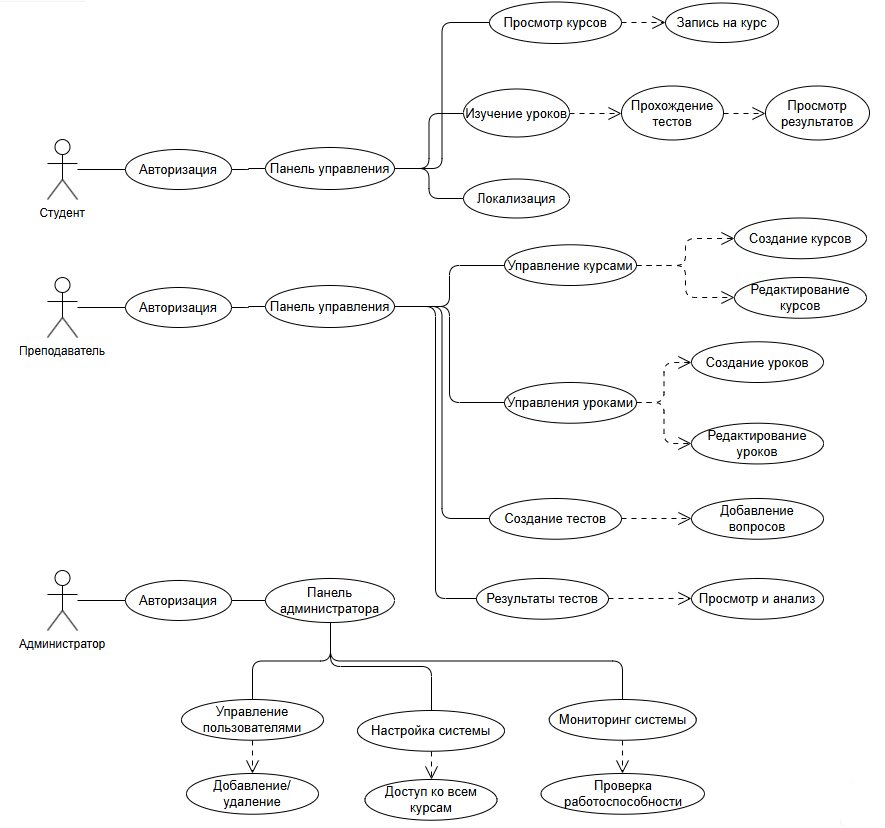
\includegraphics[width=1\linewidth]{UML}}
	\center{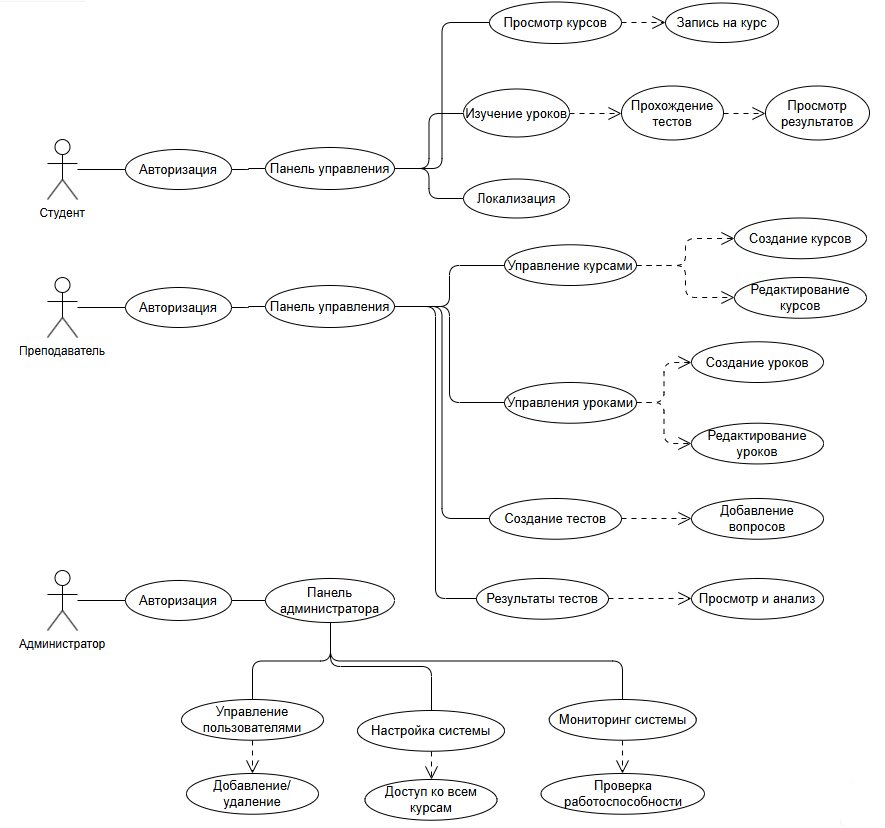
\includegraphics[width=1\linewidth]{UML}}
	\center{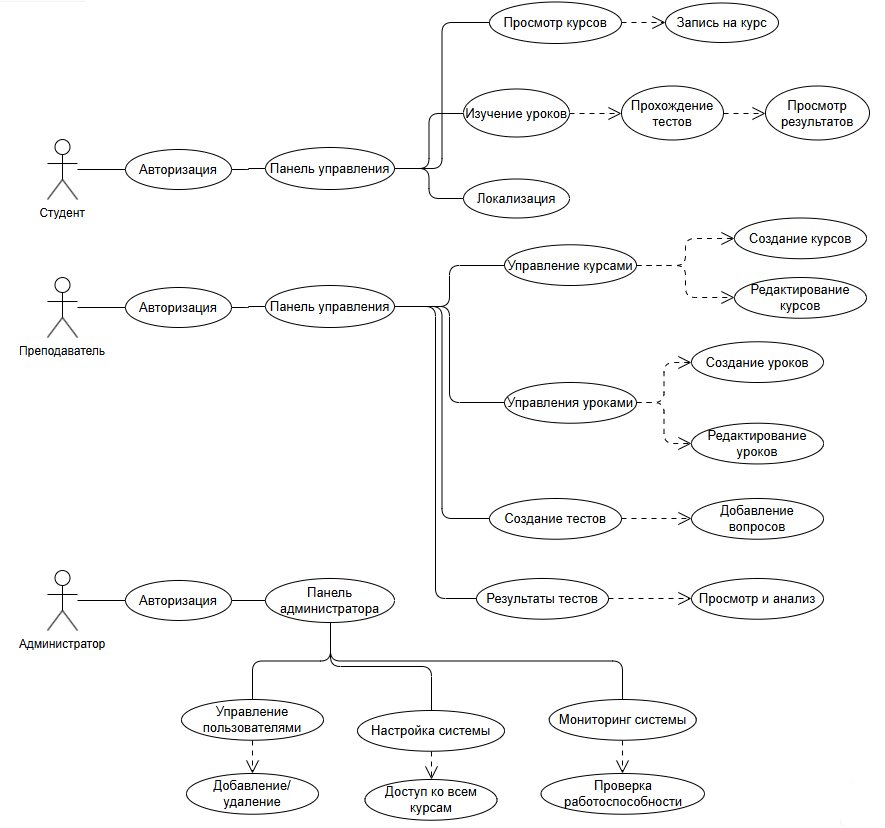
\includegraphics[width=1\linewidth]{UML}}
	\caption{Главная страница обучающей платформы}
	\label{main:image}
\end{figure}

На рисунке \ref{course:image} представлен интерфейс просмотра курса с динамическим отображением уроков и тестов по JavaScript.

\begin{figure}[ht]
	\center{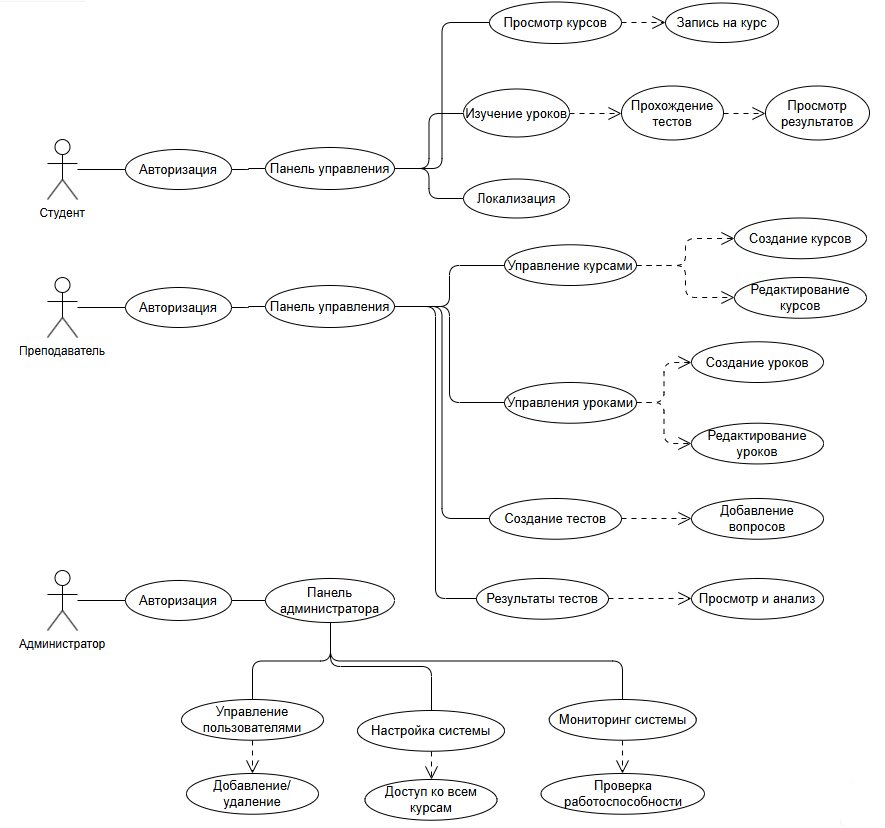
\includegraphics[width=1\linewidth]{UML}}
	\caption{Интерфейс просмотра курса}
	\label{course:image}
\end{figure}

На рисунке \ref{test:image} представлен интерфейс сдачи теста по JavaScript с динамической формой для выбора ответов.

\begin{figure}[ht]
	\center{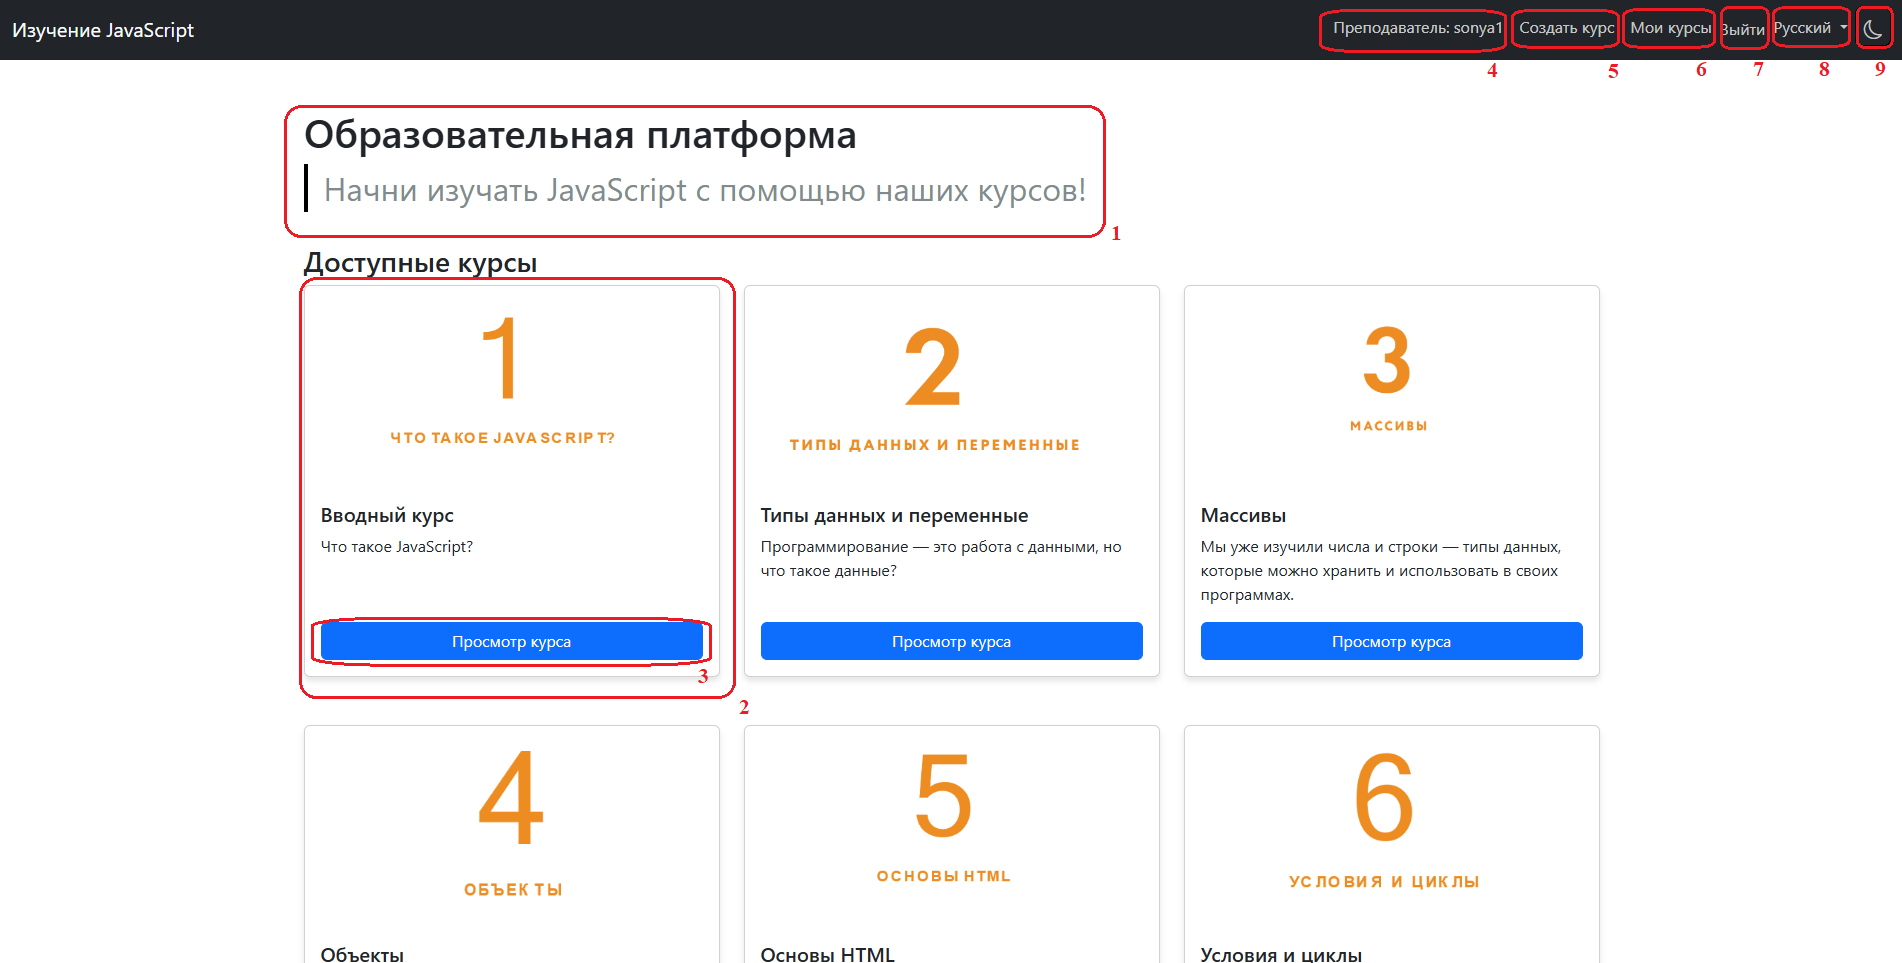
\includegraphics[width=1\linewidth]{курсы}}
	\caption{Интерфейс сдачи теста}
	\label{test:image}
\end{figure}